\section{Results and discussion}\label{sec:results}

In this section, we detail the findings of our study.  We remind the reader that our main goal with this study is the detection od blindspot that impact the false negative rate in current mining sandbox approaches and mitigating them. We hypothesize the presence of two major blindspots - dynamic call trace from the entry point to a sensitive API, and the differences in the manifest file of repackaged apps. In Section~\ref{sec:Sensitive APIs}, we summarize the results of our study that estimates the performance of Droidbot, the state of the art in mining sandbox approaches. To this end, we reproduce the approach used by DroidBot in their original paper by presenting the divergent sensitive app sets for each app pair in our dataset. We also present details regarding which sensitive APIs are accessed more commonly with malwares. 
%We also present the 
%sensitive APIs set more injected by repackaged apps, among 162 explored. 
We perform this initial study since it help solve our R1 and served as a reference to solve R2 and R3. \kn{How does this help solve R2 and R3.}

The remainder of this section is structured as follows. Section~\ref{sec:traceResults} presents the results of our study analyzing the impact of dynamic call trace on mining sandbox approaches, thereby answering R2. Section~\ref{sec:manifestResults} presents the results of our study analyzing the impact of modified manifest files on sandbox approaches, thereby answering R3. Section~\ref{sec:implications} presents some insights gained from the overall study and their potential implications.

\subsection{False negative rate and Sensitive APIs more used}\label{sec:Sensitive APIs}

In this section, we describe the results of reproducing the state-of-the-art Android sandbox approach on our new dataset of $800$ app pairs. We perform this experiment to ensure our analysis of the blind spots is done on the same playing field. Firstly, given a pair of apps, we first execute each app version using Droibot at DroidXP infrastructure for three minutes repeated three times.

After the three executions, DroidXP produces a dataset with the sensitive methods that both app versions call for each execution. We consider that a test generation tool could construct a sandbox able to detect a specific malware if there exists a sensitive method is called only by the malicious version of the app. 
%This check is done using a Python script that compares the set of sensitive methods, called at both app versions (benign/malicious).

To this end, we use DroidXP to generate reports for each execution that includes a set of observations like the set of sensitive methods accessed by each app version (benign/malicious), the sensitive methods accessed just by the malicious version (diff). If the set of sensitive methods accessed just by a malicious app is empty, this implies that the app is not marked malicious, and therefore features a false negative.

With Droidbot, our results present that it could detect a total of $193$ ($24.12$\%) where sensitive APIs set differs. The sccuracy of Droidbot here are much lower accuracy compared to those reported by previous works like Bao et al. (66.66\%)~\cite{DBLP:conf/wcre/BaoLL18}, and Costa et al. (76.04\%)~\cite{DBLP:journals/jss/CostaMMSSBNR22}. To ensure our experiments are not biased in anyway, we reproduced the results using the same smaller datasets of $102$ app pairs used by previous studies, and confirm accuracy percentages close to these previous works, ($65.3$\%). This indicates that when presented with a more representative dataset, the accuracy of DroidBot drops significantly. It is to be noted that the previous works used app pairs with a very high similarity score ($X\%$) indicating most of their apps were similar to each other. Meanwhile, our dataset has an average similarity score of ($Y\%$) with a much better distribution ($Z1\%$ of app pairs have a similarity score of less than $0.25$, $Z2\%$ of app pairs between $0.25$ and $0.50$,$Z3\%$ of app pairs between $0.5$ and $0.75$  and $Z4\%$ of app pairs more than $0.75$). 

Our exploration of all sensitive APIs called by all app pairs brought to light the most frequently abused sensitive APIs when repackaging apps. We observed that our experiments called a sensitive API for a total of $1592$ times (from our list of 162 sensitive APIs), calling at least $75$ sensitive APIs one time. $16$ APIs account for more than half of all calls ($51.06$\%). The sensitive API abused most by repackaged apps turned out to be \textbf{android.telephony.TelephonyManager: java.lang.String getDeviceId()}, which gets the device IMEI\footnote{From wikipedia: International Mobile Equipment Identity (IMEI) is a number, usually unique, to identify 3GPP and iDEN mobile phones.}. We summarize our results at Table~\ref{tab:APIused}. 

With these results, we observe that mining sandbox approaches suffer from a significantly low accuracy rate when presented with a representative dataset (higher number of app pairs and diverse similarity index), which encouraged us to endorse efforts aimed at identifying potential blindspots with such approaches and eventually answering R2 and R3.

%\begin{landscape}
\begin{table*}[t]
  \caption{Sessitive APIs more used by repackage apps}
  \centering
  \begin{small}
 \begin{tabular}{lcc}
   \toprule
   Sensitive API & Occurrences & (\%) \\
   \midrule
   01 <android.telephony.TelephonyManager: java.lang.String getDeviceId()> &  78 & 4.89 \\
   02 <android.net.wifi.WifiManager: android.net.wifi.WifiInfo getConnectionInfo()> &  64 & 4.02 \\
   03 <android.net.wifi.WifiInfo: java.lang.String getMacAddress()> &  63 & 3.95 \\
   04 <android.net.NetworkInfo: java.lang.String getTypeName()> &  58 & 3.64 \\
   05 <android.net.NetworkInfo: java.lang.String getExtraInfo()> &  56 & 3.51 \\
   06 <android.telephony.TelephonyManager: java.lang.String getSubscriberId()> &  54 & 3.39 \\
   07 <android.net.NetworkInfo: android.net.NetworkInfo State getState()> &  52 & 3.26 \\
   08 <android.database.sqlite.SQLiteOpenHelper: android.database.sqlite.SQLiteDatabase getWritableDatabase()> &  49 & 3.07 \\
   09 <android.database.sqlite.SQLiteDatabase: android.database.Cursor query(java.lang.String, ...,java.lang.String)> &  47 & 2.95 \\
   10 <android.telephony.TelephonyManager: java.lang.String getNetworkOperator()> &  45 & 2.82 \\
   11 <android.telephony.TelephonyManager: android.telephony.CellLocation getCellLocation()> &  44 & 2.76 \\
   12 <android.database.sqlite.SQLiteOpenHelper: android.database.sqlite.SQLiteDatabase getReadableDatabase()> &  44 & 2.76 \\
   13 <android.telephony.gsm.GsmCellLocation: int getLac()> &  42 & 2.63 \\
   14 <android.telephony.gsm.GsmCellLocation: int getCid()> &  42 & 2.63 \\
   
   15 <android.net.ConnectivityManager: android.net.NetworkInfo getNetworkInfo(int)> &  39 & 2,44 \\
   16 <android.telephony.TelephonyManager: java.lang.String getNetworkOperatorName()> &  36 & 2,26 \\
   .&  . & . \\
   .&  . & . \\
   .&  . & . \\
   74 <android.app.ActivityManager: java.util.List getRecentTasks(int,int)> & 1 & 0,06 \\
   75 <android.net.NetworkInfo: java.lang.String toString()> & 1 & 0,06 \\

 \bottomrule
                            Total & 1592 & 100 \\

 \end{tabular}
 \end{small}
 \label{tab:APIused}
\end{table*}
%\end{landscape}

\begin{obs}{1}{}
   %\kn{Here we need to add some final take aways of the reproduction study}
   Our results indicate that in the presence of a representative dataset ($800$ app pairs as opposed to $102$ and a diverse similarity index), the accuracy of state of the art in mining sandbox approaches, DroidBot drops significantly (from $X\%$ to $Y\%$). Our results also indicate that only few sensitive APIs are responsible for majority of injected malware in repackaged apps. This encourages the emergence of new proposals that can support mine sandbox mitigating \textit{blindspot}s that lead to low accuracy.
 \end{obs}


%\kn{In this subsection, are we simply reproducing the results of existing papers. Because as far as I understand, tools like DroidBOT etc. were evaluated by simply comparing the sensitive APIs call. I am guessing here our contribution is to evaluate it on the larger dataset. I have given it a shot, please keep me posted if this is correct.}

\subsection{Trace Analysis Results}\label{sec:traceResults}

In this section, we describe the results of our investigation on how the trace from the entry point to sensitive API could impact the accuracy of sandbox approaches. Initially, we collect the call graphs of Droidbot's execution using \emph{Logcat} and filter in the traces between the app's entry point and calls to any sensitive methods.

Then, using the callgraph from executions of both app versions (benign/malicious), we track the differences between their traces. We choose to investigate only app pairs that covered the same set of sensitive APIs detected in both versions during our first experiment (Section~\ref{sec:Sensitive APIs}). Our results show that among $607$ pair apps that had no difference between their sensitive APIs set, 176 of them ($29$\%) had different traces. This result provides evidence that thet accuracy of sandbox approaches will be improved if the traces from entry point to sensitive APIs are considered.

Table~\ref{tab:pa} summarizes the results of this investigation. The column \textbf{Same API set (SAPI)} shows the number of app pairs that had the same sensitive APIs explored at the first experiment, i.e, considered as undetected malware. The column \textbf{Trace Different (TD)} shows the number of app pairs (among the undetected ones) that have different traces from the entry point to the sensitive method. The column \textbf{Improv. \%} shows how much the malware detection of each tool could have been potentially improved if we considered the trace (calculated using ~\eqref{improve})

\begin{table}[ht!]
  \caption{Summary of the results of trace analysis. }
  \centering
  \begin{small}
 \begin{tabular}{ccc}
   \toprule
   Same API set (SAPI) & Trace Different (TD) & Improv. (\%) \\   \midrule
   607 & 176 & 22 \\
 \bottomrule
 \end{tabular}
 \end{small}
 \label{tab:pa}
\end{table}



\begin{eqnarray}
Improvement & = & \frac{trace Different (TD) \times 100}{Total App Pairs Explored} 
\label{improve}
\end{eqnarray}


Figure~\ref{fig:maliciousTrace} shows an example of trace injected in the malicious version of the app \textbf{[com.android.remotecontrolppt]}. Here, benign and malicious app versions access the same sensitive method, \textit{getSubscriberid()}. This sensitive method returns the device's unique subscriber ID, and requires the manifest file permission "READ\underline{\space}PHONE\underline{\space}STATE", present in both app version. The original app accesses this method through $2$ traces (1 and 2), which suggests an expected action from app user. However, instead of the 2 original traces, the malicious version injected a third trace containing as an entry point a method that performs a stealth computation on a background thread, \textit{doInBackground}, suggesting an action without user's awareness.\fh{explain more about this example, and find another one }

\begin{figure}
\centering
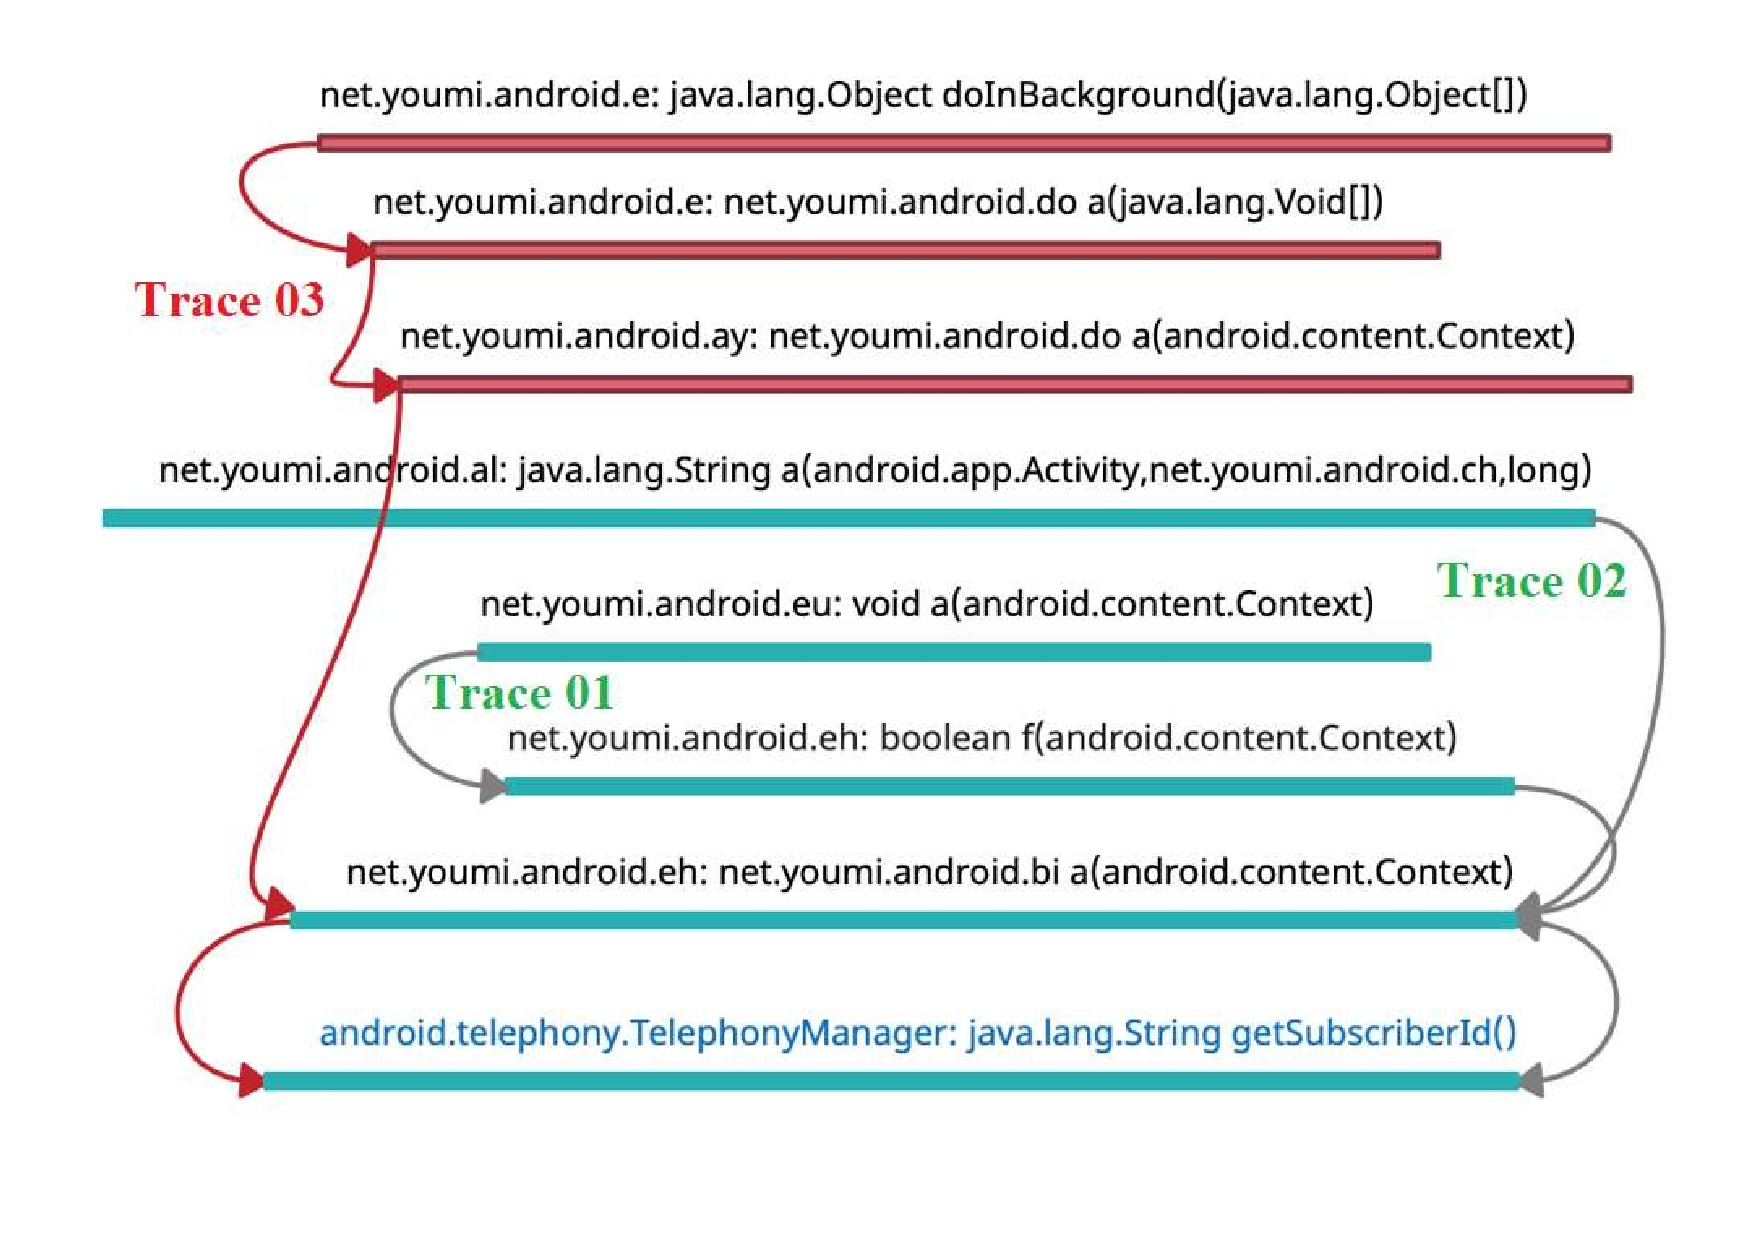
\includegraphics[scale=0.30]{images/maliciousTrace_example01.pdf}
\caption{Example of Malicious Trace.}
 \label{fig:maliciousTrace}
\end{figure}

\begin{obs}{2}{}
 Test generation tools like Droidbot have a blind-spot when it comes to being aware of the trace taken from the entry point to a sensitive API call. Droidbot could have detected $29\%$ of its undetectable malware had it considered trace as a factor.
 \end{obs}

\subsection{Manifest File Analysis}\label{sec:manifestResults}

In this section, we describe the results of our investigation on the impact of modified manifest files on the accuracy of sandbox approaches. 
To this end, we check some particulars from manifest file, that point to a likely suspicious behavior. In section \ref{sec:manifestAnalysis}, we illustrated that an automatic hacking script could inject duplicated permission and actions into the Manifest file. We looked out for such modifications in the malware that went undetected by the test generation tools. We also check if, among these apps, there were excessive requests for permissions in the malicious version's manifest files. Table~\ref{tab:mfa} and Table~\ref{tab:mp} summarizes our results. 

\begin{table}[ht]
  \caption{Manifest File with duplicate code.}
  \centering
  \begin{small}
 \begin{tabular}{ccccc}
   \toprule
   (SAPI) & (DP) & (DA) & (DP or DA) \\   \midrule
   607 & 62 & 81 & 120 \\ 
   
 \bottomrule
 \end{tabular}
 \end{small}
 \label{tab:mfa}
\end{table}

The column (SAPI) indicates the number of malware that went undetected during our first study (same as Table~\ref{tab:pa}'s Same API set (SAPI)). The second column (DP) indicates how many Manifest files had duplicated permission. Column (DA) denotes the number of malware with the duplicated actions in their manifest file.

A duplicate request for permission or action in a malicious version's manifest file should have been performed by a script. A simple analysis of manifest file could detect $120$ of undetectable malware from the first experiment ($607$), if it considers explorer duplicate permissions or actions at manifest file code as a detection strategy.

\fh{this final I do not think that is so relevant}
\begin{comment}
Finally, we investigate how many app pairs request a suspicious amount of permissions. Past works indicate that a benign Android app normally requests on average $4$ permission, while a malicious apps version requests a median number of $7$ permission\cite{DBLP:conf/soups/FeltHEHCW12}\cite{DBLP:journals/tifs/0029LBKTLC17}. To this end, we observe how many app pairs have more than a delta of $3$ permission requests in comparison with the benign version. Table~\ref{tab:mp} presents the results.

\begin{table}[ht]
  \caption{Manifest File with suspicious amounts of permission requests.}
  \centering
  \begin{small}
 \begin{tabular}{ccc}
   \toprule
   (SP) & (DP) & (NDP) \\   \midrule
   
   7 & 6 & 1 \\ 
   
 \bottomrule
 \end{tabular}
 \end{small}
 \label{tab:mp}
\end{table}

The second column (SP) presents how many app pairs not detected by the first experiment, have a suspicious amount of permission requests ($3$ or more) when compared with your benign version. 


Third and fourth columns (DP)(NDP) present how many app pairs out of these contain duplicated permission or not respectively. As we can see, just $7$ apps investigated had requested a suspicious amount of permissions, $6$ with duplicated permission in your code, and $1$ without. With these numbers we concluded that this analysis is not efficient in terms of detection of malicious activities, since, among $7$ manifest files with excessive request permission, $6$ have duplicate request permission, a suspicious behavior already detected at the first approach.

\end{comment}

\begin{obs}{3}{}
 We can conclude that sandbox approach also could have better accuracy if they considered the suspicious modifications in manifest file in their analysis. Although the analysis required of the manifest file is quite naive, we believe the results present an interesting and relevant insight for developers of malware detection tools to improve accuracy.
\end{obs}

\subsection{Implications}\label{sec:implications}

The results presented so far have implications for both practitioners and researchers. We bring evidence that there are blindspots in Android sandbox approaches that if considered as a factor in malware identification, could improve mine sandbox technique. In a first step, we present that in our study, the accuracy of sandboxes approach was slightly lower than in previous work. That is because our data set encompasses a wider range of malware, not considered in previous works. Our study points out that when using Droidbot to explore sensitive APIs at both versions, it was able to identify $193$ sensitive APIs set differents ($24.12$\%). We also show that among all sensitive APIs explored, \textbf{android.telephony.TelephonyManager: java.lang.String getDeviceId()} was the sensitive API more injected at the malicious app, responsible by $78$ calls among $1592$ at our experiment ($4.89\%$)

Next, we present a trace analysis at our data set which aims to investigate if there were some different traces between an entry point and a call to any sensitive resource. We investigated traces in which we got different sensitive APIs set from the first study. Our findings indicate that the trace analysis is also effective for malicious apps identification, and could support mine sandbox approach. Our First study had significant trace support when investigating the app pair with the same sensitive APIs explored. Among $607$ app pair investigated, we present that $176$ had different traces ($29\%$), featuring therefore as a suspicious app. The message from these findings is that exploring trace analysis in conjunction with mine sandbox approach is useful for researchers and practitioners to improve malicious app detection tasks. 

Finally, the last study used static analysis at Android manifest files, to investigate if even naive techniques to construct malicious apps can go unnoticed for mine sandbox approach. In the previous section, Table~\ref{tab:mp} and~\ref{tab:mfa} summarizes this investigation. Although seems to be a simple technique, we reported some suspicious manifest files from malicious apps which also was a blindspots in Android sandbox approaches. The static analysis on manifest files revealed that among $607$ app pair, $120$ considering duplicated permissions or actions in manifest file.

For industry and academia, these results have implications. They reinforce that there are benefits of integrating auxiliary techniques to mine sandbox approach for malware identification. We also present evidence that its possible benefit from static analysis on suspicious Android manifest files for malware identification, even at malware with a low similarity coefficient regarding its benign version. If we consider both integrated approaches, our accurate rate in terms of malware detection grows from ($24.12\%$) to ($55.75\%$) in our real-world dataset (800 app pair), ($22\%$) for the first approach, and ($9.63\%$) for the second.

The Venn-diagram of Figure~\ref{fig:vennDiagram} present the number of malicious app detected by Sensitive APIs Diff approach, by trace analysis, and by two kinds of suspicious manifest files, as well as how they complement each other.

\begin{figure}[ht]
\centering
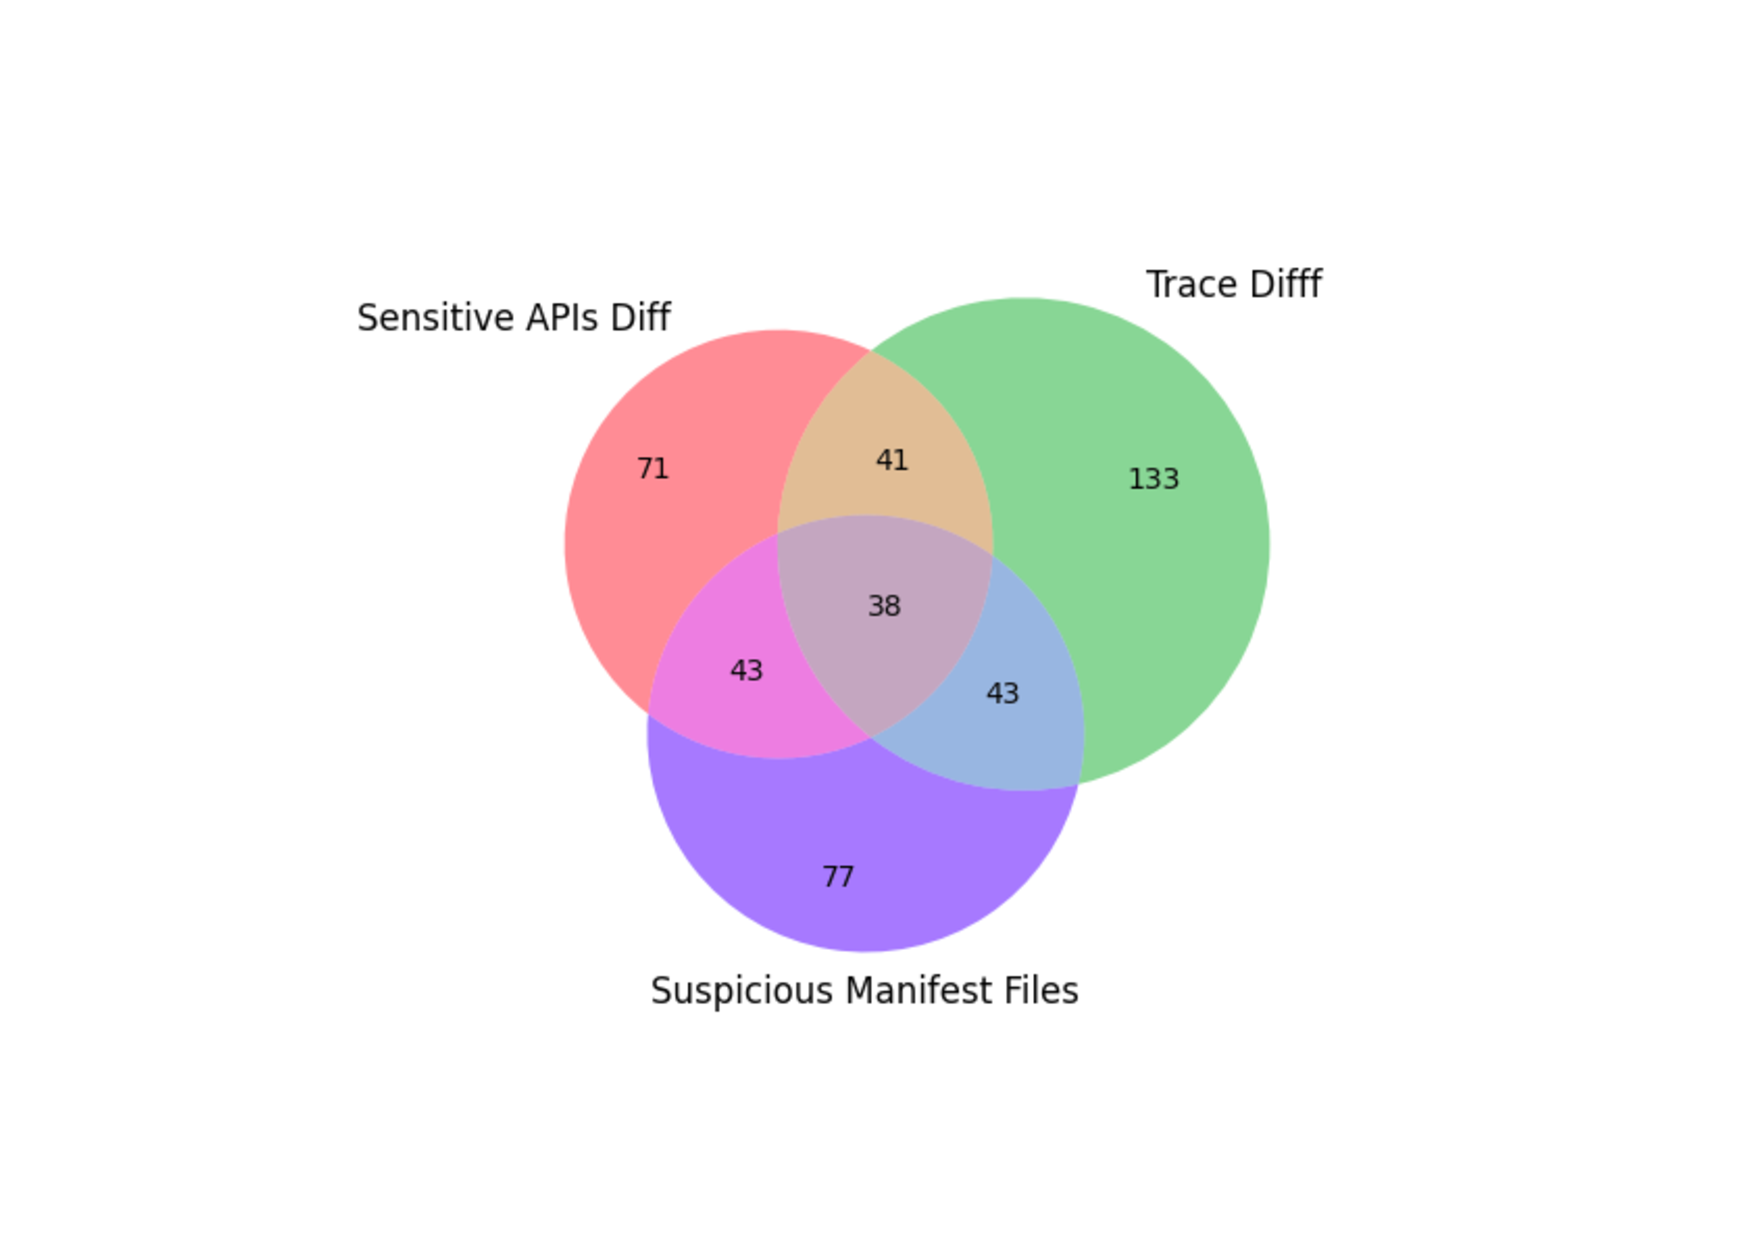
\includegraphics[scale=0.35]{images/vennDiagram.pdf}
\caption{Venn Diagram from results.}
 \label{fig:vennDiagram}
\end{figure}


%\fh{Here we have to insert a venn-diagram based at our file summaryAll.csv}